\section{Evaluationsprotokoll}
\label{sec:evalprotokoll}

\subsection{Warum der frühere temporale Split ersetzt wurde}

Die erste Auswertung verwendete innerhalb jedes Experiments eine zeitliche 80/10/10-Aufteilung. Im Fall der Autoaufnahmen lagen die Testframes damit am Ende der Trajektorie. Splitzugehörigkeit und Objektposition waren gekoppelt.

Konkret hatte das bewegte Auto in den letzten zehn Prozent der Aufnahme den gut einsehbaren Bereich bereits verlassen. Das Testsegment enthielt das Zielobjekt also kaum noch oder nur stark verdeckt. Der sehr niedrige damalige dynamische Auto-AP\textsubscript{30} von \(\texttt{os1}=0{,}09\) beschrieb somit nicht die allgemeine Qualität von \texttt{os1}, sondern die Generalisierung auf diesen letzten räumlichen Trajektorienabschnitt.

Dieser Befund darf nicht mehr als Hauptresultat verwendet werden. Die Cross-Validation mit vollständig zurückgehaltenen Experimenten ersetzt den temporalen Split als wissenschaftliche Hauptbewertung.

\subsection{Experiment-held-out Cross-Validation}

Das Protokoll wurde am 11. Juli 2026 vor der Sichtung der Cross-Validation-Testergebnisse eingefroren \cite{raschka2018model}. Abbildung~\ref{fig:cv-fold-diagramm} gibt einen Überblick über das Schema.

\begin{figure}[H]
\centering
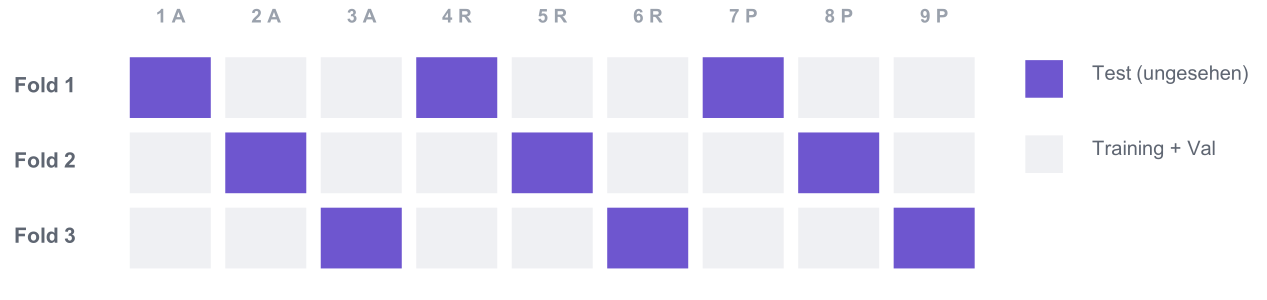
\includegraphics[width=\textwidth]{images/cv-fold-diagramm.png}
\caption[Schema der experiment-held-out Cross-Validation]{Experiment-held-out Cross-Validation: Jedes Experiment wird in genau einem Fold getestet, die übrigen dienen mit einem zeitlichen Guard dem Training und der Validierung.}
\label{fig:cv-fold-diagramm}
\end{figure}

Die drei Folds sind in Tabelle~\ref{tab:cv-folds} zusammengefasst:

\begin{table}[H]
\centering
\begin{tabular}{cc}
\toprule
\textbf{Fold} & \textbf{Vollständig ungesehene Testexperimente} \\
\midrule
1 & Auto~1, Fahrrad~4, Person~7 \\
2 & Auto~2, Fahrrad~5, Person~8 \\
3 & Auto~3, Fahrrad~6, Person~9 \\
\bottomrule
\end{tabular}
\caption{Experiment-held-out Cross-Validation: Zusammensetzung der drei Folds.}
\label{tab:cv-folds}
\end{table}

Innerhalb der jeweils übrigen sechs Experimente werden die letzten zehn Prozent als Validierungsdaten verwendet. Die zehn davorliegenden Frames pro Trainingsexperiment werden als zeitlicher Guard ausgeschlossen. Die vollständigen Testexperimente werden weder für das Training noch für die Checkpoint-Auswahl verwendet. Tabelle~\ref{tab:cv-split-counts} gibt die resultierenden Frame-Anzahlen pro Fold wieder.

\begin{table}[H]
\centering
\begin{tabular}{ccccc}
\toprule
\textbf{Fold} & \textbf{Training} & \textbf{Validierung} & \textbf{Test} & \textbf{Guard} \\
\midrule
1 & 1.239 & 146 & 677 & 60 \\
2 & 1.172 & 137 & 753 & 60 \\
3 & 1.227 & 143 & 692 & 60 \\
\bottomrule
\end{tabular}
\caption{Frame-Anzahlen pro Fold nach Training, Validierung, Test und Guard.}
\label{tab:cv-split-counts}
\end{table}

Alle drei Ansichten erhalten pro Fold identische physische Zeitstempel. Damit ist der View-Vergleich zeitlich gepaart. Die bereits erwähnten ansichtsspezifischen Labels bleiben jedoch erhalten.

\subsection{Metriken}

Eine Vorhersage gilt als Treffer, wenn ihre dreidimensionale Intersection over Union (IoU) mit einer noch nicht zugeordneten Ground-Truth-Box derselben Klasse den betrachteten Schwellwert erreicht. Verwendet werden AP\textsubscript{30}, AP\textsubscript{40}, AP\textsubscript{50} und AP\textsubscript{60}:

\begin{itemize}
    \item AP\textsubscript{30} bewertet überwiegend, ob das Objekt ungefähr gefunden wurde.
    \item AP\textsubscript{60} verlangt eine deutlich präzisere räumliche Lokalisierung.
    \item Der Klassen-mAP mittelt über AP\textsubscript{30} bis AP\textsubscript{60}.
    \item Der Gesamt-mAP mittelt zusätzlich über die drei Klassen.
\end{itemize}

Die tiefgestellten Zahlen bezeichnen durchgehend die IoU-Schwelle in Prozent. Die AP selbst wird als datensatzweite, elfpunktinterpolierte AP berechnet. Vorhersagen werden nach ihrem Konfidenzscore sortiert; Matching bleibt frameweise, die Precision-Recall-Kurve wird jedoch aus der gesamten Testmenge aufgebaut.

\subsection{Fold-Mittel und gepoolte Out-of-Fold-Auswertung}

Die Fold-Ergebnisse sind die primäre Generalisierungsschätzung. Aus ihnen werden Mittelwert und Stichproben-Standardabweichung berechnet. Zusätzlich werden die Vorhersagen aller drei Testfolds zu einer gepoolten Out-of-Fold-Auswertung zusammengeführt. Dabei wurde jeder Frame genau von dem Modell vorhergesagt, für das sein vollständiges Experiment ungesehen war.

Die gepoolte AP wird einmal auf der gemeinsamen Rangliste aller Out-of-Fold-Vorhersagen berechnet. Sie ist deshalb nicht identisch mit dem arithmetischen Mittel dreier AP-Werte. Da die Konfidenzscores der drei Foldmodelle unterschiedlich kalibriert sein können, ergänzt der gepoolte Wert die Foldanalyse, ersetzt sie aber nicht.

\subsection{Offizielle und labelbasierte Auswertung bewegter Objekte}

Die offizielle dynamische Teilbewertung ignoriert eine Vorhersage auf einem statischen Objekt nur, wenn diese am jeweiligen Evaluationsschwellwert ausreichend mit der statischen GT-Box überlappt. Eine etwas ungenau lokalisierte, aber eindeutig einem geparkten Auto zuordenbare Box kann dadurch bei AP\textsubscript{60} als False Positive der dynamischen Rangliste erscheinen.

Deshalb existiert zusätzlich eine benannte labelbasierte Variante. Sie nutzt das manuelle \texttt{static}-Attribut und ignoriert Vorhersagen auf Nichtzielobjekten bereits ab IoU 0{,}25. Die regulären All-Object-Metriken bleiben dabei bit-identisch; nur die Teilranglisten für bewegte und statische Objekte ändern sich. Die offizielle Auswertung bleibt die Vergleichsreferenz, während die labelbasierte Variante die interpretierbare Analyse der bewegten Objekte liefert.

Zur Offenlegung gehört, wie diese Variante entstanden ist. Sie wurde nicht gemeinsam mit dem Cross-Validation-Protokoll eingefroren, sondern erst nach der Analyse des in Abschnitt~\ref{sec:ap60-artefakt} beschriebenen AP\textsubscript{60}-Artefakts definiert. Ihre Wirkung fällt zugunsten der fusionierten Ansicht aus und zeigt damit in Richtung der untersuchten Hypothese. Aus diesem Grund gelten drei Festlegungen: Die offizielle Auswertung bleibt unverändert dokumentiert und behält den Status der Vergleichsreferenz, jede Angabe aus der labelbasierten Variante wird als solche gekennzeichnet, und die Regel wird für alle drei Ansichten identisch angewendet. Alle zentralen Ergebnisse werden deshalb unter beiden Varianten berichtet (Tabellen~\ref{tab:bewegt-fold} und \ref{tab:alle-schwellen}). Im aggregierten Bewegt-mAP bleibt die Rangfolge der Ansichten in beiden Varianten dieselbe. Auf der Ebene einzelner Klassen und Schwellen können sich Werte und Rangfolge dagegen unterscheiden; am deutlichsten beim bewegten Auto, wo die offizielle Variante \texttt{os0} vorn sieht und die labelbasierte \texttt{merged}. Beim Fahrrad sind beide Varianten identisch, weil in den Daten keine statischen Fahrräder annotiert sind.
